%\documentclass[letterpaper,oneside]{article}
% letterpaper,10pt,oneside,onecolumn,final
\documentclass[hidelinks]{article}

\usepackage{cmap}
\usepackage[T1]{fontenc}
\usepackage[utf8]{inputenc}
\input glyphtounicode
\pdfgentounicode=1

\usepackage[english]{babel}
\usepackage[backend=biber,style=numeric,sorting=none]{biblatex}
%\addbibresource{hops-spec.bib}

\usepackage{adjustbox}
\usepackage{graphicx}
\usepackage{amsmath}
\usepackage{amsfonts}
\usepackage{amssymb}
\usepackage{subcaption}
\usepackage{hyperref}
\usepackage{listings}
\usepackage{csquotes}
\usepackage{textcomp}
\usepackage{outlines}
\usepackage{enumitem}

\usepackage{algorithm}
\usepackage{algpseudocode}
\renewcommand{\algorithmicrequire}{\textbf{Input:}}
\renewcommand{\algorithmicensure}{\textbf{Output:}}

\usepackage{placeins}

\usepackage[printwatermark]{xwatermark}
\newwatermark[pages=1-12,color=gray!25,angle=45,scale=5,xpos=0,ypos=0]{DRAFT}


\let\Oldsection\section
\renewcommand{\section}{\FloatBarrier\Oldsection}

\let\Oldsubsection\subsection
\renewcommand{\subsection}{\FloatBarrier\Oldsubsection}

\let\Oldsubsubsection\subsubsection
\renewcommand{\subsubsection}{\FloatBarrier\Oldsubsubsection}

\makeatletter
\newcommand\urlfootnote@[1]{\footnote{\url@{#1}}}
\DeclareRobustCommand{\urlfootnote}{\hyper@normalise\urlfootnote@}
\makeatother


\usepackage{color}



%\usepackage{lineno}
%\linenumbers

\definecolor{dkgreen}{rgb}{0,0.6,0}
\definecolor{gray}{rgb}{0.5,0.5,0.5}
\definecolor{mauve}{rgb}{0.58,0,0.82}

\definecolor{lightgray}{gray}{0.75}




\usepackage{graphicx}
\usepackage{amsmath}
\usepackage{amsfonts}
\usepackage{amssymb}
\usepackage{multirow}
\usepackage{subcaption}
% \usepackage{lineno}
\usepackage{listings}
\usepackage{microtype}
\usepackage{placeins}
\usepackage[x11names]{xcolor}
\usepackage{footnote}


\usepackage[T1]{fontenc}
\usepackage[scaled]{beramono}
\newcommand\Small{\fontsize{9}{9.2}\selectfont}
\newcommand\Normal{\fontsize{12}{12.3}\selectfont}
\newcommand*\LSTfont{\Small\ttfamily\SetTracking{encoding=*}{-60}\lsstyle}
\newcommand*\LSTfontNormal{\Normal\ttfamily\SetTracking{encoding=*}{-60}\lsstyle}


\usepackage{listings}


\lstset{ %
  backgroundcolor=\color{white},   % choose the background color; you must add \usepackage{color} or \usepackage{xcolor}
  basicstyle=\LSTfont,        % the size of the fonts that are used for the code
  breakatwhitespace=false,         % sets if automatic breaks should only happen at whitespace
  breaklines=true,                 % sets automatic line breaking
  captionpos=b,                    % sets the caption-position to bottom
  commentstyle=\color{gray},    % comment style
  deletekeywords={...},            % if you want to delete keywords from the given language
  escapeinside={\%*}{*)},          % if you want to add LaTeX within your code
  extendedchars=true,              % lets you use non-ASCII characters; for 8-bits encodings only, does not work with UTF-8
  frameshape={RYR}{Y}{Y}{RYR},	                   % adds a frame around the code
  keepspaces=true,                 % keeps spaces in text, useful for keeping indentation of code (possibly needs columns=flexible)
  keywordstyle=\color{blue},       % keyword style
  language=C++,                 % the language of the code
  otherkeywords={*,...},           % if you want to add more keywords to the set
  numbers=none,                    % where to put the line-numbers; possible values are (none, left, right)
  numbersep=5pt,                   % how far the line-numbers are from the code
  numberstyle=\tiny\color{gray}, % the style that is used for the line-numbers
  rulecolor=\color{black},         % if not set, the frame-color may be changed on line-breaks within not-black text (e.g. comments (green here))
  showspaces=false,                % show spaces everywhere adding particular underscores; it overrides 'showstringspaces'
  showstringspaces=false,          % underline spaces within strings only
  showtabs=false,                  % show tabs within strings adding particular underscores
  stepnumber=2,                    % the step between two line-numbers. If it's 1, each line will be numbered
  stringstyle=\color{red},     % string literal style
  tabsize=2,	                   % sets default tabsize to 2 spaces
  title=\lstname                   % show the filename of files included with \lstinputlisting; also try caption instead of title
}


\usepackage{tabularx}
\newcolumntype{L}{>{\raggedright\arraybackslash}X}


%\usepackage{tikz}
%\usepackage{pgfplots}
%\usetikzlibrary{positioning}
%\usetikzlibrary{shapes.geometric, arrows}
%\pgfplotsset{compat=1.11}
\usepackage[margin=0.9in]{geometry}

\newcommand\tikzmark[2]{%
  \tikz[remember picture,overlay]\node[arrow,draw] (#1) {#2};}


%\usepackage[printwatermark]{xwatermark}
%\newwatermark[pages=2-30,color=gray!25,angle=45,scale=5,xpos=0,ypos=0]{DRAFT}

\usepackage{etoolbox}
\makeatletter
\patchcmd{\@verbatim}
  {\verbatim@font}
  {\verbatim@font\tiny}
  {}{}
\makeatother

\usepackage{ifthen}

\let\endtitlepage\relax

\newcommand{\FIXME}[1]{{\bf {\color{red} #1}}}
\newcommand{\nuHOPS}{{\bf {\color{dkgreen} (new)HOPS}}}

% Title Page
\title{ \textbf{MSRI HOPS Re-development Specification} }
\author{
\large Geoff Crew, John Barrett, Dan Hoak, Violet Pfieffer \\
\Large MIT Haystack Observatory}
\date{Draft - Version 1.0, \today}


\begin{document}
\maketitle

%\vspace{1.5in}

\tiny
\tableofcontents
\normalsize
\newpage
%\listoffigures
%\newpage
%\listoftables
%\newpage

%   * Architecture definition
%   * Language selection
%   * Build system selection
%   * Parallel support definition
%   * Interactivity definition
%   * External package identification
%   * New objects specification
%   * New library specification
%   * New program specification
\section{Introduction}

This document is intended to record the design decisions made in specifying how the HOPS re-development project undertakes the
re-design and re-implementation of the VLBI post-processing software HOPS. As this is a software project there is a certain
degree of ongoing flexibility that is needed in order to obtain an optimal result upon completion. Therefore, this 
draft document will be updated periodically along with the software as it is built out. The initial focus will be to determine
the of components of the design and their dependencies which must be in place as basic infrastructure before further development
can take place.


\section{General Architecture}

The goal of the re-developed HOPS architecture is provide a component-based design which allows for a greater degree of flexibility
in the types of operations that may be applied to VLBI data during fringe fitting, and avoid the semi-monolithic approach used in the past.
To do this, the software package to be delivered will primarily comprise of a set of loosely coupled libraries which can be composed
into an variety of calibration and fringe-fitting applications. Moreover, rather than attempting to identify and categorize all manner of data
types and data manipulation which may be required by future observations at the outset, a primary goal of this project is to provide a
relatively flexible set of data containers and operators along with a python plugin interface so as to allow for future extensions with minimal revision to the existing code.

For the foreseeable future, the main source of input data to this software will be provided by the DiFX correlator. However, this may not always
be the case, so in order to decouple the correlator from the post-processing software a conversion utility must be provided. This follows
the same paradigm as the current code, where a separate application (difx2mark4, which depends on the DIFXIO library) handles the conversion. However,
in this iteration we propose that this conversion utility operate mainly as a transparent pass-through, merely
converting the correlator output into the native post-processing data format, rather than applying any initial calibration/normalization (e.g. auto-corrs) or
other corrections to the data.

Once the data has been converted to the native post-processing format additional manipulation within the fringe-fitter will take place in several stages, such as normalization, data-flagging, a priori phase/delay and band-pass calibration, and finally fringe search. At intervening stages
both the data objects and data operator objects will be exposed to a python interface and hooks will be provided for external user scripts to 
access and directly modify the data and/or data operators. A extremely simplified diagram of the control flow of such a single-baseline fringe-fitter executable is shown in \ref{fig:fringe-fitter}. A multi-baseline global fringe-fitting algorithm will also be made possible by refactoring the HOPS code, however, the exact nature of this algorithm (e.g. Cotton-Schwab or baseline stacking, etc.) and whether it will best be implemented as a configurable option of a single fringe-fitting executable or as its own separate exectuable needs to be determine.

Upon completion of fringe fitting, the calibrated data with fringe solution applied will then be saved in a native binary format with the option to convert to an archival format (e.g. HDF5) via a simple conversion utility. Intermmediate stages (with partial data corrections applied) may also optionally saved to the native format. It is also desired that
the export of a data flagging table and band-pass correction table be made possible, such an export tool may initially be implemented via user python script. If a multi-package (HOPS/AIPS/CASA) exchange format is adopted/secified then this feature could be made a built-in option in the refactored code.

In addition to the fringe fitter itself, a number of other post-fringing data analysis tools will also be provided. Most importantly are
a fringe plot utility for diagnostic information about the quality of an individual fringe, as well as the equivalent executables to \textit{alist} and \textit{aedit}, which summarize multiple fringe solutions and display condensed information about multiple scans respectively.
We intended to preserved the existing functionality of these executables, but expect to make the fringe-plot more flexible by providing options
to enable/disable various plotting items.


\begin{figure}[h!]
\begin{center}
  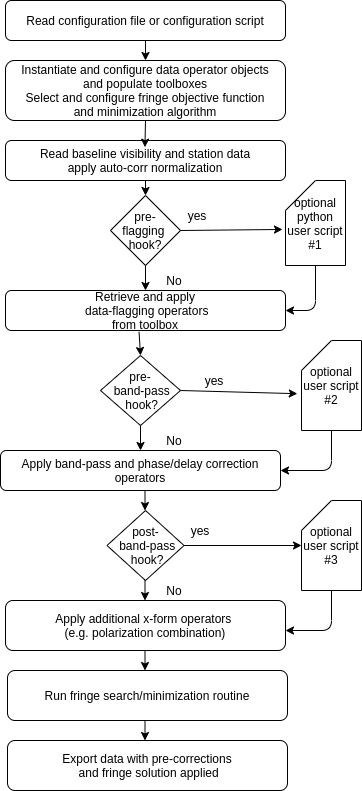
\includegraphics[width=0.6\textwidth]{example-single-baseline-fringe-fitter.png}
    \caption{Example of simplified control flow for a single-baseline fringe fitter.}
    \label{fig:fringe-fitter}
\end{center}
\end{figure}



% Design language choices
\section{Language, Build and Version Control System}

Several aspects need to be taken into account when deciding on a choice of programming language for this project. Namely, some of these are:
\begin{enumerate}
 \item Availability of software developer expertise.
 \item The inherent performance attainable with a specific language.
 \item Availability of high performance open source utility libraries for math, I/O, etc.
 \item The primary language of the existing code base (C).
 \item The accessibility and ease of extensibility of the project by users with varying levels of experience
\end{enumerate}

Obtaining a reasonable balance between these considerations is difficult with a single language. Therefore we
plan to develop a multi-language project, wherein the base computation layer is handled within C/C++,
but additional data manipulation can be done via optional Python plugins embedded within the aapplication
or independently by external Python scripts which have access to some of the underlying application libraries.
C++ is a good choice given current personnel and developer expertise, and being a super-set of the C language
it provides the ability to reuse of portions of the existing C code base with little to no change, while also adding modern language features
(templates, classes and inheritance, const. correctness, function overloading, etc.). A combined C/C++ approach
allows for much easier memory management (currently handled rather painfully in the existing HOPS code base) and also
enables the use of a wide variety of open source libraries, not least of which is the built in standard template library
which provides access to a wide collection of basic data types (strings, vectors, maps, etc) and algorithms (searching, sorting, etc.)
which will reduce the required amount of maintenance of internal code and reliance on external libraries.

Further augmenting C/C++ libraries with inter-language communication to Python can be done via a wide variety of mature tools
(ctypes, boost.Python, SWIG, pybind11, etc.), and will increase the ease at which outside users can augment the software without
needing to have expertise in C/C++/. Since Python 2 is no longer supported, all new development will be Python 3.

The build system for this project will be automake\urlfootnote{https://www.gnu.org/software/automake/} or CMake\urlfootnote{https://cmake.org}, and version control will proceed through a locally hosted (Haystack) git repository. HOPS3 used the automake build system and there is some
advantage in re-using that frame work, while the CMake build system is generally easier to maintain than the current automake system when faced with the complexities of a multi-language project. It also allows for a more user-friendly configuration at the time of compilation, as the user can be presented with a menu providing options which are dependent on the available set of tools/libraries that are currently installed and detected on the users system. Initially
both build systems may be implemented to see which provides an optimal choice. While version control will be handled in a local \textit{git} repository during
the prime development phase, it is expected that eventually a public \textit{git} repository will be made available for releases which will also make it much easier to leverage community contributions if so desired at some point in the future.


\section{Objects specification}

\label{sec:objects}


Generally speaking the code will be organized around roughly three object type categories involved in the structure of the new HOPS. These are as follows:

\begin{enumerate}
 \item Meta Data Containers: These serve to store small quantities of station and baseline metadata associated with an observation of disparate types.
 \item Array Containers: These serve to organize large n-dimensional arrays of a single data type (e.g. visibility data and correction/calibration table data). 
 \item Data Operators: These evaluate a function or perform some transformation on a given data container. Their operation is configurable via a set of exeternally defined parameters, while their application to any particular data set can be made conditional by a set of filters.).
\end{enumerate}

\subsection{Data Containers}

The existing HOPS3 code base relies on a fixed number of \texttt{C} structs to organize and present the data related to an observation. The strict memory layout of these structures has the advantage of making them cross-machine compatible, which is necessary since these structures are also used as the core components of the Mark-4 I/O library. However, a notable disadvantage of this rigid design is the degree of difficulty encountered in making changes to the existing data structures, or adding new data types in order to accommodate additional information which was not originally envisioned at the time the library was written. To make the data structures more flexible we intend to decouple the in-memory data layout from the file I/O, so they do not necessarily need to be byte-for-byte copies.

\subsubsection{Meta-Data Containers}

In a strictly typed language such as \texttt{C}, flexible data structures have a high degree of code overhead, not only in the management of dynamic memory allocation, but more severely in the conversion of data types and typecasting. To ameliorate this we propose to exploit \texttt{C++11}'s variadic template mechanism, which allows for the transformation of type-agnostic class lists into concrete class types or hierarchies at compile time. This makes it possible to store disparate types (so long as the complete set of types is known at compile time) within in the same object that are indexed and can be retrieved by the same type of key (e.g. a name string). Listing \ref{lst:metaobjects} gives a condensed example of the preliminary version of the template base class for a meta-data container (with detailed functionality removed).

\lstinputlisting[language=C++,label={lst:metaobjects},caption=Meta-data object template classes for multi-type maps.]{code/metadata-objects.hh}

To the extent possible, the in-memory meta-data structures should be classes which provide access via a key-value pair mechanism so as to avoid exposing the private internal storage layout to the routines needing access to subsets of the data. This retrieval mechanism also has the benefit of completely decoupling the compile
time structure of the data containers from the data they need to hold at runtime. A key:value interface is trivially available via the STL std::map template class,
so there is no need to expend effort on a native implementation. Moreover this sort of interface should also make conversion of these data structures into widely accessible formats such as JSON or python dictionaries possible for data export to external software.

\subsubsection{N-Dimensional Array Containers}

We propose the following basic set of class templates be used to construct most in-memory objects used for the manipulation of correlated observation data and its associated station data:
\begin{enumerate}
 \item ScalarContainer - encapsulates scalar-like data 
 \item VectorContainer - encapsulates vector-like data
 \item TableContainer - encapsulates rank-N tensor-like data with associated axes (vector)
\end{enumerate}
These template classes are to serve as a simple wrapper around the management of the raw memory needed to store a data item and keep track of its associated unit(s), 
and (if applicable) the values associated with the axes along each dimension and their units.

Listing \ref{lst:objects} gives a brief sketch of the preliminary class template implementation for these data container objects, while listing \ref{lst:visib} gives a simple example of what template declaration of an object storing visibility data from an observation over single baselines and polarization products might look like.
A graphical representation of a TableContainer is shown in figure \ref{fig:table-container}.

\lstinputlisting[language=C++,label={lst:objects},caption=Data object templates]{code/data-objects.hh}

\lstinputlisting[language=C++,label={lst:visib},caption=Visibility object type]{code/visibilities.hh}


\begin{figure}[h!]
\begin{center}
  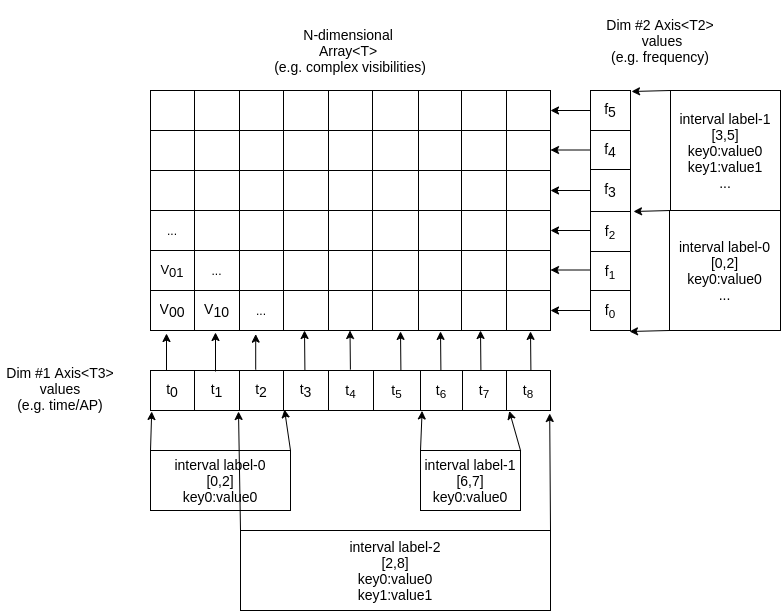
\includegraphics[width=\textwidth]{data-container-baseline.png}
    \caption{A graphical representation of a TableContainer. This class is composed of an N-dimensional array, coupled with axes to provide coordinate values
    along each dimension. The axes themselves allow for arbitrary intervals to be labelled by key:value pairs in order to allow for local look-up of filter data.
    For example, along the frequency axis, the interval labels may be channel or sampler names among other possibilities. Furthermore, the interval and associated
    labels will be stored in an interval-tree stucture to allow for fast bi-directional lookup of data indices $\leftrightarrow$ data labels.}
    \label{fig:table-container}
\end{center}
\end{figure}

\subsection{Data operators}

The data operator classes are meant to organize the mathematic manipulations which are to be performed on the data containers. For example, many of the operations performed in the existing HOPS3 code-base (such as the application of a priori phase calibration) are relatively trivial linear transformations applied to the visibility data. However, they are currently intertwined with a large amount of control logic which obscures the basic data pathway (e.g see postproc/fourfit/norm\_fx.c)
Most unary or binary operations that are to applied to visibility or other data residing in TableContainers such as scaling, multiplication, transposition, summation, Fourier transformation, etc. will be made available as individual classes inheriting from the same interface. A uniform class interface will allow these data operators to be composed or modified to create more complicated composite operators or strung together to accomplish data pipelines of arbitrary complexity. An additional advantage of encapsulating individual operations is that any SIMD parallel-processing extension used to accelerate data processing can be made opaque to the user.

Listing \ref{lst:operators} gives a brief sketch of the class templates generalizing the data operators. The common inheritance from the base class \texttt{MHO\_DataOperator} allows them all to be stored in an common comtainer so that once they are configured and initialized they may be retrieved
and executed in the appropriate order. It is expected that the vast majority of the data operators will be unary, requiring only their own configuration 
parameters and the data container upon which they operate as inputs, but we will also support binary operators accepting two data containers, an example
of which is the application of a pre-constructed calibration table to a new data set.

One aspect of the data operators which is not yet detailed here is a notion of what pieces of meta-data each operator may need in order to complete its function.
While these meta-data items could be exposed via external setter/getters, a more preferable option which would preserve encapulation would be for each operator
to define an internal schema, listing the keys and type of the parameters it needs to retrieve from the meta-data multi-type map container. 
In addition, a mechanism for filtering operations (e.g. if station = Xx, then apply this operator) also needs to be established independent of the
previous control-block structure of HOPS3.

\lstinputlisting[language=C++,label={lst:operators},caption=Data operator template classes.]{code/data-operators.hh}

\section{Parallel processing}

The existing fringe-fitting process is largely a data-parallel process operating on individual baselines with no inter-process
communication. This lends itself easily to simple parallelism using multiple independent processes (SPMD), which has been exploited
\cite{blackburn2019eht} to deal with the EHT data volume. However, this approach eliminates the ability to simultaneously fit for global or station-based
parameters and requires multiple iterations in order to apply successive calibration/corrections. Therefore, if some calibration tasks are to be
done simultaneously with fringe-fringe fitting, this will require both a substantial architectural change from the current fitting algorithm, but
also necessarily reduce the degree of (simple) parallelism available. To accommodate this, some parallel processing will have to be addressed
within the application. To do this we will use a multi-staged approach during the course of development.

Initially, the software to be developed under this project will focus on a simple single-threaded implementation, whereupon careful
profiling will inform us of the largest computational bottlenecks. For example, in the current HOPS code the majority of
the computation time is spent in a single routine (vrot.c, which is essentially just evaluating a complex exponentian and multiplying two complex numbers) that is applied over
a large array of data. This sort of task can easily be parallelized on modern multi-core architectures using the SIMD approach. We propose to use OpenCL
for this purpose given its support on a wide variety of architectures (mult-core CPUs, GPUS, hardware accelerators, etc.).

This type of parallelism exploits vector instructions and/or multiple processors to execute the similar operations over wide swaths of data. while given current experience with the existing HOPS leads us to expect that SIMD parallelism should largely be adequate to accelerate fringe fitting, if during the process of development it is discovered that a thread-based model (MIMD, where each parallel thread follows a semi-independent code pathway) could be more advantageous, then we propose to use OpenMPI framework to implement this. The reason being, that while OpenMPI does have a larger development overhead than most other threading libraries (e.g. pthreads, c++11 threads, etc.) it can be easily scaled beyond a single computer when and if needed. However, it should be noted that by necessity, any OpenMPI implementation must be developed as an independent executable (although it would be able to take advantage of any available libraries and SIMD policies present). 


\section{External Package Selection}

To the extent possible the software to be developed in this project should make all external dependencies optional whenever possible. That is to say, that
while some features may be missing if an optional external package is missing, the core functionality of the software should not be affected. For example, if the fast Fourier transform library FFTW3 is missing, the code should fall back to an internal implementation (which is allowed to be slower), but which produces equivalent output. Likewise, while an effort should be made to support portability of the output data into useful downstream formats (HDF5), this should not preclude a
basic native format capable of storing the same data for fallback, development, and debugging purposes.

The following table is a preliminary list of which external packages are expected to be incorporated as required or optional dependencies. If an optional package is missing on a user's machine the software will default to a fallback option (if available) or disable the features which require that particular package.

\begin{center}
\begin{table}[h!]
\begin{adjustbox}{width=\textwidth}
\begin{tabular}{|c|c|c|c|}
\hline
Name & Optional/Required? & Purpose & Fallback option \\ \hline
C++11 STL & Required & Standard template library & None \\ \hline
Python &  Required & Scripting language interpreter & None \\ \hline
SWIG or pybind11 & Required & C/C++ $\leftrightarrow$ Python interface and bindings & None \\ \hline
OpenCL & Optional & SIMD parallelism & Single-threaded implementation \\ \hline
OpenMPI & Optional & MIMD parallelism & Single-threadd implementation \\ \hline
FFTW3 & Optional & fast Fourier transform acceleration & native code \\ \hline
GSL & Optional & Linear algebra and special functions & TBD native code \\ \hline
HDF5 & Optional & File input/output & TBD native binary format \\ \hline
matplotlib & Optional & Python plotting library & None \\ \hline
difxio & Required & DiFX I/O library - needed for file converter only & None \\ \hline
\end{tabular}
\end{adjustbox}
\caption{List of optional/required dependencies.}
\label{tab:dep}
\end{table}
\end{center}

\section{Interactivity and Interfaces}

Interactivity with the user will proceed primarily through a python scripting interface. This avoids the need to develop a separate scripting language, 
as the python interpreter can be embedded in the application. Access to library objects will be exposed via python bindings, so that a user may have direct access 
to the data containers and operators, and can implement external routines to modify the data. Real-time interactivity via CLI or GUI is 
not planned to be implemented. We intended to preserve the functionality of the existing \texttt{fourfit} control file input method, however, this
is primarily for backwards compatibility and regression testing, no new features will be made available via this mechanism.

\section{Libraries and executables}

\subsection{Libraries}

The libraries of this project are currently broken down by task into the following modules:

\begin{enumerate}
     \item Utilities - Commonly used utilities (e.g. date handling, profile timers, etc.)
     \item Math - Math routines: linear algebra, minimizers, interface to optional 3rd-party math libraries (FFTW,GSL).
     \item Message - Controls the topic and verbosity level of application messages/logs to user.
     \item Containers - In-memory data containers of visibility and meta-data and native format I/O.
     \item MK4Interface - Allows for import/export to legacy MK4-types for testing and backwards compatibility.
     \item Operators - Base classes for data manipulation, and generic operations (array reduction, summation, transposition, FFT, etc.).
     \item VLBI - VLBI task-specific data operators (e.g. band-pass correction, per-channel phase offsets, etc.)
     \item Bindings - Python interface to C++ data containers and operators. Allows for python script configuration of data 
     operators at initialization, and user-defined direct access/manipulation of the data.
    \item  Legacy c-libraries (made available for re-use and backwards compatibility and to provide the legacy fourfit application)
    \begin{enumerate}
        \item mk4util - utility library for MK4 data types
        \item dfio - I/O for MK4 data types
        \item afio - I/O library for alist manipulation
        \item ffcontrol - parse old-style fourfit control files 
        \item ffcore - core parameter structures
        \item ffio - output for fringe file data
        \item ffmath - trivial math routines used by fourfit
        \item ffplot - fringe-plot generation library 
        \item ffsearch - core fringe-search algorithm library (grid-search)
    \end{enumerate}
\end{enumerate}

An additional set of plugin libraries will be enabled if the appropriate dependencies are present at compile time, as follows:

 \begin{enumerate}
    \item DIFXInterface - depends on difxio and converts the correlator data into the native data container format.
    \item HDF5 I/O - Converts the native data objects to/from an archival HDF5 file.
    \item Plotting - Utilities to generate plots for data exploration (e.g. fringe-plots). This will be implemented in python.
    \item SIMD extensions (OpenCL) - Parallel implementation of some set of the data operators.
 \end{enumerate}


\begin{figure}[h!]
\begin{center}
  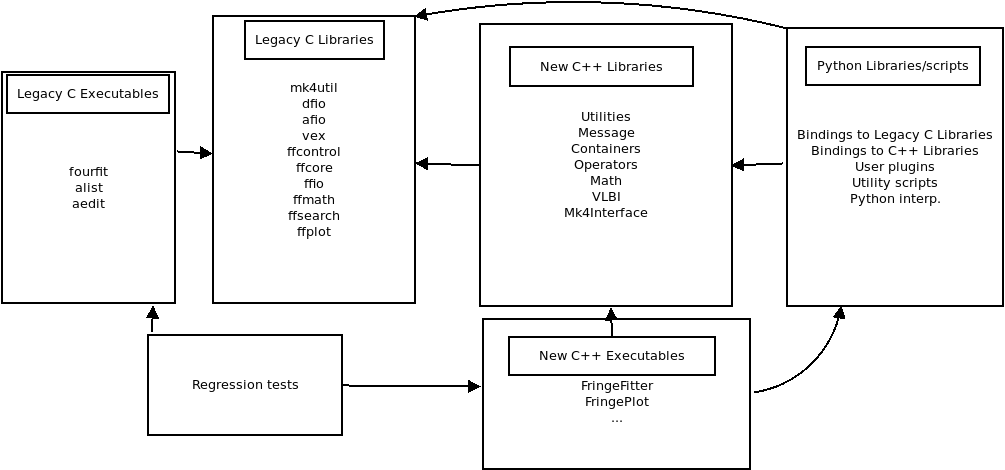
\includegraphics[width=0.95\textwidth]{arch_overview.png}
    \caption{Basic overview of library and executable dependency architecture. Arrows indicate direction of dependency (from child to parent). Shaded boxes are new to-be-developed software.}
    \label{fig:lib-arch}
\end{center}
\end{figure}


\subsection{Executables}

The executables to be delivered will largely be composed through the re-use of the library code and at a minimum will consist of the following (though not necessarily
named as such):

\begin{enumerate}
 \item DiFX2Input  - difx2mark4 equivalent, converts correlator (difx) data into native input format.
 \item Station utilities  - converts station calibration data (e.g. ANTAB) files into native input format.
 \item FringeFitter - fourfit-replacement, accepts a user script (or old-style control file backwards compatibility) for configuration and direction and applies user specified procedures to the visibility data.
 \item FringePlot  - plotting tool, creates fringe-plots and all graphical data exploration.
 \item HDF5Export  - converts any native formats into an HDF5 format for access by external programs.
 \item DataInspect - data inspection tool, dumps data objects to a human readable format.
 \item alist - data inspection tool, dumps simple fringe summary data to a human readable format (as in HOPS3).
 \item aedit - data inspection/visualizatoin tool (re-coded in python), reads alist files and provides simple plots of multple scan data (as in HOPS3).
 \end{enumerate}

%
% section to cover legacy code
%
\section{Legagy Software}

The transition from HOPS 3 to HOPS 4 is sufficiently disruptive that proper
regression from the old tools to the new tools (with enhance functionality)
needs preservation.  As part of the migration from the SVN repository (that
supported HOPS 3 development) into the GIT repository (that supports HOPS 4
development) there is an opportunity to retain code that might prove useful
to the ngEHT effort.  As a practical necessity, the EHT must function as a
working array during the HOPS 4 development, so there may also be additional
changes to HOPS 3 (bug fixes) or critical functional patches (i.e., bandpass
correction for NOEMA).

Consequently, the GIT repository will contain copies of the HOPS 3 code to
allow regression testing.  This also mitigates against development slip in
that code that might otherwise be overhauled for future extension may continue
to function as it currently exists.  This is particularly true of A-list based
processing where major format changes are not likely (or which would be
encapsulated within the afio library).

To avoid confusion, applications that bear the same name (so that scripts may
still continue to function) shall follow the Python 2 to 3 migration approach
where a 3 or a 4 is appended to the executable name.  A user-selectable
configuration option then allows to specify which version is used for the
original name.  (I.e.,
\texttt{python} gets you 
\texttt{python2} or 
\texttt{python3}, depending on user choice.)

A second reason for this approach is that modified/developmental versions may
in some cases leverage existing code (not yet rewritten) which allows for
functional versions of many of the applications of the package prior to the
completion of the rewrite.  This allows use of HOPS 4 with EHT data prior to
completion of the project.  This is not intended for science use (use of
un-released code is not allowed) but rather as part of our effort to continue
to assess the development of HOPS 4.

Applications that we expect to survive in legacy form likely includes:
\texttt{adump},
\texttt{aedit},
\texttt{alist},
\texttt{average},
\texttt{cofit},
\texttt{fourfit},
\texttt{fourmer},
\texttt{fplot},
\texttt{fringex},
and
\texttt{search}.

%
% eof
%
 

%
% above to be deleted after merger
%
\newpage
\addtocounter{section}{1}
\renewcommand{\refname}{\thesection. References}
%\bibstyle{plainurl}
%\bibliography{hops-spec}





\end{document}
